\newacronym{api}{API}{Application Programming Interface}
\newacronym{json}{JSON}{JavaScript Object Notation}
\newacronym{jdk}{JDK}{Java Development Kit}
\newacronym{url}{URL}{Uniform Resource Locator}

\section{External Source}\label{sec:external_source}
An alternative method of Context enrichment is based on acquiring concept definitions from external sources, especially when these are not already available as metadata annotations in the ontologies that are validated. The lookup is solely based on the concept's name, neglecting the connected nature of an ontology. Dictionaries have always been the first choice when it comes to searching for specific information about words or phrases. We chose \textit{WordNik}\footnote{\url{https://www.wordnik.com/} accessed 2018/06/15} as source for external content, a freely available online dictionary for the English language. Among other features that were offered, we used \emph{example sentences} that were collected from various sources across the Web. 

This section begins with a brief introduction into WordNik, the online dictionary we used for the provision of example sentences, and then continues with our approach of using WordNik as content provider for concept descriptions.   


\subsection{WordNik}\label{sec:wordnik}
WordNik targets native English speakers who look up words that are rare~(technical terms or dialect terms), very old or very new. They often search for definitional information which is incomplete or missing in traditional dictionaries. Users tolerate published imperfection because they opt for relevant, actual and cutting-edge information, even though not officially approved by editors~\cite{burnett1979}. They want to understand the context of word usage in sentences, not necessarily explanatory statements as in printed or even online dictionaries.

The driving force behind WordNik was contribution. It processes and aggregates external user-generated content such as tweets, newspaper articles, scientific articles or uploaded Flickr\footnote{\url{https://www.flickr.com/} accessed 2018/06/15} images. This is similar to what search engines do, but with restricted scope. The creators of WordNik observed that very few people write word definitions, they rather add meta linguistic information such as lists of their favourite words, comments or tags. WordNik additionally collects statistics about lexicographical terms, more or less frequently searched words and most commented words. 

WordNik also offers an \gls{api} for programmatically accessing their resources\footnote{\url{https://developer.wordnik.com/} accessed 2018/06/15}. Besides the word definition, it also provides access to audio metadata, etymology, word usage, syllable information, bi-gram phrases, text pronunciations, relation diagrams to other words, example sentences and others. At the time of writing this thesis free access is granted for non-profit, non-commercial use with a limitation on the number of \gls{api} calls. 
After a successful registration process, an \gls{api} token is provided which is a prerequisite for \gls{api} interaction. Besides Web access, a handful of libraries\footnote{\url{https://developer.wordnik.com/libraries} accessed 2018/06/15}, available in many programming languages, were created to facilitate integration with third-party applications. 

\subsection{Dictionary based Approach}\label{sec:enrichment_dictionary_approach}
Intuitively, the idea of generating descriptions using dictionary lookup is simple: starting from a concept name, descriptions are built from consulting the online dictionary \hyperref[sec:wordnik]{WordNik}. 

A schematic overview of the overall workflow is shown in~\hyperref[fig:external_source_workflow]{Figure~\ref*{fig:external_source_workflow}} and described below:
\begin{figure}
	 \centering
	 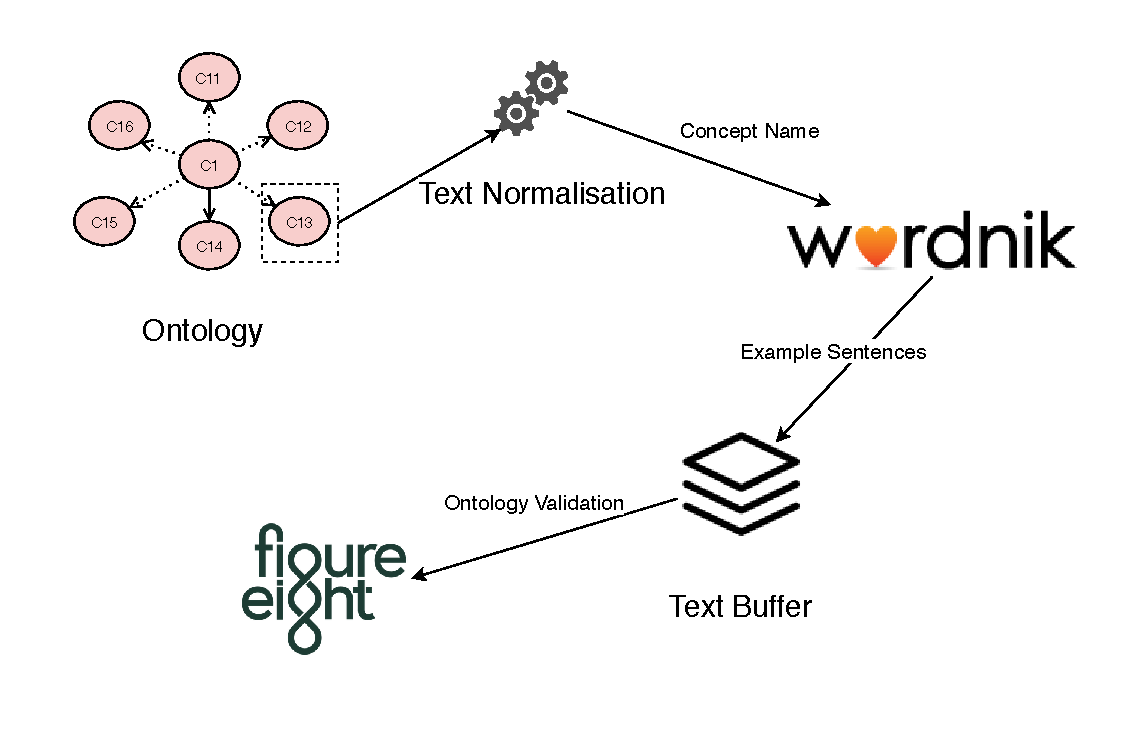
\includegraphics[width=0.9\textwidth]{drawio/External_Source_Workflow}
	 \caption{Conceptual workflow of WordNik consultation to generate concept descriptions}\label{fig:external_source_workflow}
\end{figure}

\begin{enumerate}[label=\textbf{[Step \Roman*]},leftmargin=\widthof{[Step III]}+\labelsep]
	\item \emph{(Concept Selection)} The first step in the workflow is the selection of the concept(s)
	      for generating the description. For that, the ontology engineer selects the concept(s) and
		  starts the enrichment process. 
	\item \emph{(Text Normalisation)} The idea is to use the concept name as a baseline for any further
	      processing. Often, the name can not be used directly as input to WordNik because it
		  contains unwanted characters such as excessive spaces, quotes, dots or just non-printable
		  characters. This is especially true for learned ontologies, generated from textual sources.
		  Our algorithm uses the built-in text manipulation capabilities of the \gls{jdk} to pre-process
		  concept names.
	\item \emph{(Dictionary Lookup)} Next, WordNik is consulted to find example sentences for normalised
	      concept names. In contrast to traditional dictionaries, WordNik searches in all kinds of available
		  online content, including newspapers, journals, scientific publications, tweets and others. All
		  \gls{api} interaction is protected against unauthorised access, however, to help developers learning
		  the \gls{api}, some features are available in isolated Sandbox~Mode\footnote{\url{https://developer.wordnik.com/docs} accessed  2018/06/21} 
		  too.
		  
		  For example, when searching for the word \guillemotright chartjunk\guillemotleft~which does not
		  have a definition in traditional dictionaries, the \gls{api} response is illustrated
		  in~\hyperref[lst:WordNik_response_for_chartjunk]{Listing~\ref*{lst:WordNik_response_for_chartjunk}}. The
		  output is encoded in \gls{json}\footnote{\url{https://tools.ietf.org/html/rfc7159} accessed 2019/01/05}
		  which defines a common, human-readable format for data transmission. The example shows one \emph{example
		  sentence}~(the others were omitted because they share the same structure) including various other
		  properties besides the actual title and text. Our algorithm just skips these other properties because they were
		  not needed for the final concept description. However, it might be useful in certain scenarios to differentiate 
		  between duplicate entries by exampleId or exploring further details by adding the source \gls{url}.
	\item \emph{(Text Buffering)} Depending on wether a single concept or multiple concepts are validated, example sentences
	      need to be harmonised, which is realised by storing intermediate results and mapping these to the initial concepts.
	\item \emph{(Crowdsourcing Submission)} The last step of the workflow is the creation of the questionnaire for the actual
	      ontology validation. As for all enrichment methods, the only part that varies for each approach is the concept
		  description, shown as top part of the template.
		  \hyperref[fig:wordnik_example_questionaire]{Figure~\ref*{fig:wordnik_example_questionaire}} depicts the
		  questionnaire presented to crowd workers for the example from above.
\end{enumerate}

\begin{lstlisting}[frame=single,breaklines=true,postbreak=\mbox{\textcolor{black}{$\hookrightarrow$}\space},caption=WordNik \gls{api} response for the word \guillemotright chartjunk\guillemotleft,label=lst:WordNik_response_for_chartjunk]
	{
	  "examples": [
	    {
	      "provider": {
	        "name": "spinner",
	        "id": 712
	      },
	      "year": 2008,
	      "rating": 185,
	      "url": "http://www.emersonprocessxperts.com/archives/2008/10/improving_how_y.html",
	      "word": "chartjunk",
	      "text": "Marshall described \"chartjunk\" as additional graphics not related to the data in a quest to make the chart more aesthetically pleasing.",
	      "title": "Emerson Process Experts",
	      "documentId": 15463705,
	      "exampleId": 289744774
	    },
		...
	  ]
	}
\end{lstlisting}

\begin{figure}
	 \centering
	 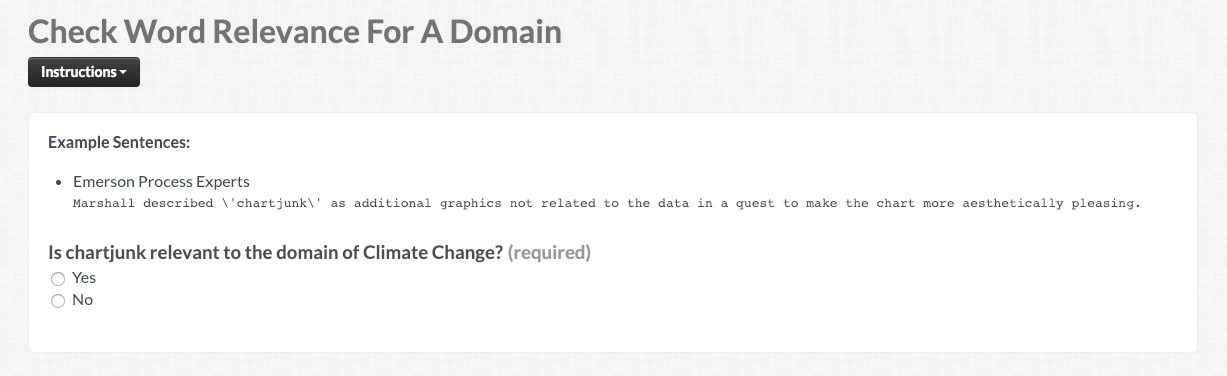
\includegraphics[width=\textwidth]{screenshots/questionaire_wordnik_example}
	 \caption{Questionnaire presented to crowd workers for searching \guillemotright chartjunk\guillemotleft~on WordNik}\label{fig:wordnik_example_questionaire}
\end{figure}
